\section{\textbf{Marco Te\'orico}}
En la \'ultima d\'ecada, ha surgido un enorme inter\'es acerca de llevar a cabo tareas de mineria de datos sobre series temporales \cite{dataminingtimeseries}. Literalmente, cientos de art\'iculos han introducido nuevos algoritmos para indexar, clasificar, segmentar y agrupar series temporales \cite{sigmod}. Es por lo anterior, que iniciamos el desarrollo del marco te\'orico definiendo series temporales, como una pieza de conocimiento angular, para la comprensi\'on y la defici\'on del contexto de nuestra propuesta de tesis.
\subsection{Series Temporales}
Las series temporales, pueden definirse como: \textit{\enquote{una secuencia de N observaciones (datos) ordenadas y equidistantes cronol\'ogicamente, sobre una caracter\'istica (serie univariable o escalar) o sobre varias caracter\'isticas (serie multivariable o vectorial), de una unidad observable, en diferentes momentos}} \cite{tak-chung}.\par
Una representaci\'on matem\'atica com\'un de una serie temporal \textit{univariable} puede verse de la siguiente manera:\par
$y_1, y_2,...,y_N; (y_t)^N t=1; (y_t:t=1,...,N)$, donde $y_t$ es la observaci\'on $n^0$ $t(1 \leq t \leq N)$ de la serie y N es el n\'umero de observaciones que componen la serie completa (el tama\~no o la longitud de la serie) \cite{concepts}.\par
En el siguiente gr\'afico, se pueden observar algunos ejemplos de las diferentes formas que pueden adoptar las series temporales, con respecto a la naturaleza de la fuente de datos que se est\'a representando. Algunas son m\'as predecibles y constantes, mientras que otras fluctuan con mayor frecuencia en amplitud o simplemente presentan mayor cantidad de ruido.
\begin{center}
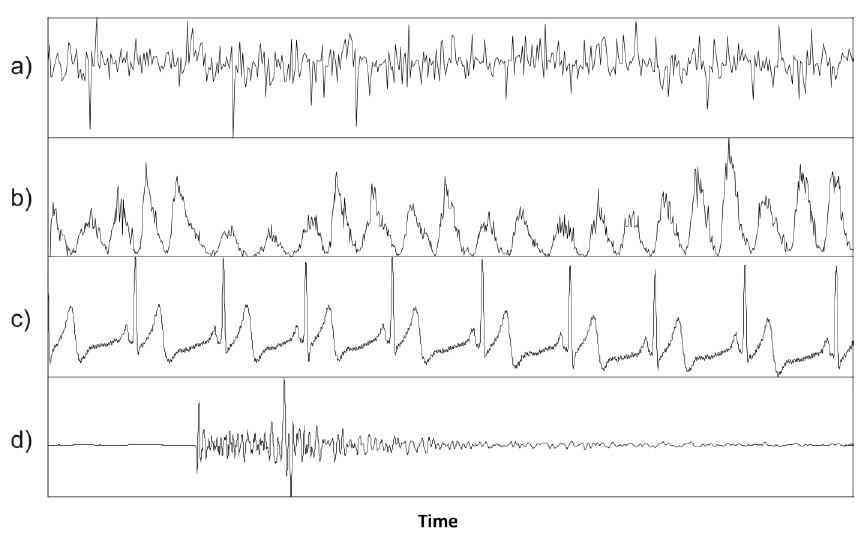
\includegraphics[scale=0.7]{timeSeries.png}
\vspace*{10pt}
\footnotesize{
\begin{tabular}{l}
\textbf{Figura 1.} Ejemplo de la representaci\'on en series temporales de: \textbf{a)} Monz\'on, \textbf{b)} Manchas Solares,\\ \textbf{c)} Electrocardiograma, \textbf{d)} Se\~nales S\'ismicas. \textbf{Fuente:} \cite{concepts}.
\end{tabular}}
\end{center}
A diferencia de las series temporales no estarionarias ilustradas en el gr\'afico anterior, muchas series temporales tienen una tendencia creciente, por ejemplo, el n\'umero de autom\'oviles en uso de un pa\'is, durante los \'ultimos cincuenta a\~nos, o decreciente como el n\'umero de personas que trabajan en la agricultura. Existen muchas otras, sin embargo, que no tienen tendencia y son estacionarias, por ejemplo, la luminosidad a horas sucesivas, que var\'ia c\'iclicamente a lo largo de las 24 horas del d\'ia \cite{concepts}.\par
La representaci\'on matem\'atica m\'as frecuente de una serie temporal multivariable, puede definirse de la siguiente manera:\\
$y_1, y_2,...,y_N; (y_t)^N t=1; (y_t: t=1,...,N)$, donde $y_t \equiv [y_t1, y_t2,...,y_tM]' (m \geq 2)$ es la observaci\'on $n^0$ $t(1 \leq t \leq N)$ de la serie y N es el n\'umero de observaciones que conforman la serie completa.\par
Las observaciones pueden ser almacenadas en una matriz $Y$ de orden $N x M$, como se muestra a continuaci\'on en la siguiente imagen:\\
\begin{equation}
Y \equiv \kbordermatrix{
				 & {    } \\	
				 & {y'_1} \\
				 & {y'_2} \\
				 & {.}    \\
				 & {.}    \\
 				 & {.}    \\
 				 & {y'_N} \\
		} \equiv
\kbordermatrix{
				 & {    }  & {    }   & {     } & {     } & {     } & {     }\\	
				 & {y'_{11}} & {y'_{12}}  & {  .  } & {  .  } & {  .  } & { y_{1M}}\\	
				 & {y'_{21}} & {y'_{22}}  & {  .  } & {  .  } & {  .  } & { y_{2M}}\\	
				 & {.}     & {.} &  &  &  & {.} \\
				 & {.}     & {.} &  &  &  & {.} \\
 				 & {.}     & {.} &  &  &  & {.} \\
 				 & {y'_{N1}} & {y'_{N2}} & {.} & {.} & {.} & {y_{NM}}  \\
}
\end{equation}\\
donde $y_{tj}$ es la observaci\'on $n^0$ $t(1 \leq t \leq N)$ sobre la caracter\'istica o variable $n^0$ $j(1 \leq t \leq N)$, que es la misma en todo momento $t$ \cite{concepts}.\\\par
Una vez definido el concepto de series temporales y como se explicar\'a m\'as adelante durante el desarrollo de este documento, la presente propuesta de investigaci\'on, se enfoca principalmente en el uso de \enquote{Cubic Spline Interpolation} como medida de distancia incorporada en dos algoritmos. Ambos algoritmos analizan los conjuntos de datos en forma de series temporales, para la identificaci\'on y la selecci\'on de \enquote{reglas significativas}. \par 
Una \textit{\enquote{\textbf{regla significativa}}} debe entenderse como un patr\'on o \enquote{subsecuencia recurrente} de la serie de tiempo (usualmente llamado \textit{\textbf{\enquote{motif}}}), que describe un evento o comportamiento real del conjunto de datos que est\'a siendo analizado. Una vez que el motif ha sido identificado, se debe analizar su capacidad predictiva en relaci\'on con el flujo de datos. Se debe tener presente entonces, el hecho de que no todas las reglas motif identificadas ser\'an seleccionadas como significativas \cite{main}.\par
\subsection{An\'alisis y Aplicaciones de Series Temporales}
El an\'alisis de las series temporales, en general, podr\'ia verse como la medici\'on, el seguimiento y el estudio del comportamiento de alg\'un fen\'omeno o  actividad en el tiempo, con el objetivo final de encontrar conocimiento relevante \cite{algoanalysis}. El resultado de dicho an\'alisis, es conocimiento de primera mano, que puede ser utilizado para comprender mejor aquello que ha venido ocurriendo. Es posible tambi\'en, a trav\'es del an\'alisis, monitorear el estado actual de las series temporales, para explicar la relaci\'on causal o la estructura subyacente que producen los datos observados. Finalmente, es completamente viable adem\'as, realizar predicciones o pron\'osticos, que podr\'ian proveer un control anticipado probable, sobre el fen\'omeno estudiado \cite{main}.\par
Por otra lado, existen innumerables aplicaciones e implementaciones existosas de la miner\'ia de datos sobre series temporales \cite{concepts}. Por ejemplo, en el campo de la medicina, un epidemi\'ologo podr\'ia estar interesado en analizar, mediante reglas significativas, el n\'umero de casos de influenza observado durante un per\'iodo de tiempo. De igual forma, a trav\'es de la trazabilidad y el an\'alisis de las mediciones de la presi\'on arterial de un individuo, se podr\'an anticipar complicaciones asociadas con mayor precisi\'on, conduciendo a una mejor evalua\-ci\'on de los medicamentos utilizados en el tratamiento de ese mal \cite{timeseriesapplications}. De igual manera, los patrones resultantes de una resonancia magn\'etica funcional de las ondas cerebrales (en forma de series temporales), pueden ser utilizados para vaticinar las reacciones cerebrales ante ciertos est\'imulos menores \cite{timeseriesapplications}. Finalmente, las aplicaciones m\'as intensivas y sofisticadas en el an\'alisis de series temporales, se enfocan en la resoluci\'on de problemas asociados a ciencias f\'isicas y ambientales. Por ejemplo, el an\'alisis de los niveles de contaminaci\'on de una regi\'on, el seguimiento de la temperatura global, el an\'alisis de la actitividad s\'ismica, el reconocimiento de vos, entre muchos otros \cite{timeseriesapplications}.\par
A continuaci\'on, se exponen algunas de las principales dificultades y retos que podr\'ian presentarse durante las diferentes etapas del proceso de miner\'ia de datos sobre series temporales.
\subsection{Grandes Retos Sobre la Miner\'ia de Series Temporales}
El an\'alisis y el descubrimiento de patrones sobre series temporales, por definici\'on, presenta una serie de retos y complicaciones que deben abordarse, tales como: la super multidimensional, la presencia de grandes cantidades de datos que muchas veces resultan innecesarios o poco \'utiles durante el an\'alisis, la sensibilidad al ruido o a la presencia de valores at\'ipicos y el dinamismo durante la transmici\'on de datos o \textit{\enquote{data streaming}}, debido a que se requiere en todo momento una gran capacidad de c\'omputo de datos, para analizar las fluctuaciones constantes sobre el conjunto de datos \cite{main}.\par
En adici\'on a lo anterior, \textit{\textbf{el c\'alculo de la similitud}} durante la comparaci\'on de dos o m\'as series temporales es considerado un desaf\'io a\'un mucho m\'as crucial en la miner\'ia de series temporales, especialmente cuando se ha realizado previamente una reducci\'on de la dimensionalidad, de la escala o la amplitud a trav\'es del tiempo. La carencia de un alineamiento oportuno sobre el eje tiempo o la amplitud, durante el c\'alculo de la similitud entre dos o m\'as series temporales, es un problema serio debido a que ocasiona un impacto directo sobre el resultado de la comparaci\'on. \cite{concepts}.\par
El c\'alculo de la similitud es indispensable en la identificaci\'on de segmentos re-petitivos, contenidos en la serie de tiempo. Dichos segmentos se denominan reglas \textit{\textbf{\enquote{motifs}}} o \textit{ocurrencias frecuentes de un subconjunto de la serie temporal} \cite{main}.\par
Los motifs pueden considerarse conocimiento significativo, cuando, como producto del an\'alisis del flujo de datos de la serie temporal, se pueden utilizar para predecir un fen\'omeno o evento con una alta probabilidad \cite{main}.\par
La idenficaci\'on de reglas \textit{motif} se logra fundamentalmente apartir del c\'alculo de las medidas de distancia entre los elementos de dos o m\'as series temporales \cite{main}; la precisi\'on de dicho c\'alculo y el n\'umero de ocurrencias son vitales para determinar la calidad de dicha regla. Existen en la literatura, un n\'umero importante de medidas de distancia \cite{distancecomparison}. Las medidas de distancia m\'as importantes para la comprensi\'on de esta propuesta ser\'an desarrolladas a continuaci\'on.
\subsection{Medidas de Distancia para el C\'alculo de la Similitud}
Las medidas de similitud son de vital importancia cuando se ejecutan tareas de an\'alisis y miner\'ia de datos sobre series temporales, tales como: descubrimiento de patrones, agrupamiento, clasificaci\'on, descubrimiento de reglas, anal\'is de valores at\'ipicos, entre otras \cite{concepts}.\par
Debido a la naturaleza n\'umerica y continua de de los datos caracter\'isticos de las series temporales, las medidas de similitud, t\'ipicamente se llevan a cabo en forma de aproximaciones \cite{distancecomparison}.\par
Los estudios existentes sobre series de tiempo se basan en cuatro categor\'ias de funciones de distancia \cite{measurements}. La primer categor\'ia consiste en las \textit{Lp-normas} o \enquote{\textit{Lp-norms}}. Son funciones de distancia m\'etricas o lineales, que no soportar cambios en el desplazamiento local del eje tiempo, por ejemplo, la distancia Euclideana o la distancia Manhatthan. La segunda categor\'ia, por otra parte, se conoce como \textit{medidas el\'asticas}, y consisten en funciones de distancia capaces de lidiar con desplazamientos locales en el eje tiempo, pero no son m\'etricas o lineales. La categor\'ia tres, son medidas de distancia basadas en un umbral (por ejemplo TQuEST \cite{distancecomparison}). Por \'ultimo, la categor\'ia cuatro corresponde a todas aquellas medidas de distancia basadas en la \textit{\enquote{forma}} o en un patr\'on de la serie temporal, tal es el caso de SpADe \cite{spade}. \par
La complejidad inherente al c\'alculo de las medidas de similitud, imponen normalmente las principales limitaciones y restricciones de capacidad y tiempo de c\'omputo, sobre los algoritmos utilizados en el an\'alisis y la miner\'ia de datos de series temporales \cite{algoanalysis}. Es decir, cuanto m\'as r\'apido y preciso sea el c\'alculo de la medida de similitud definida en el algoritmo, menor ser\'a el tiempo de c\'omputo necesario para la ejecuci\'on del procedimiento completo de miner\'ia de datos sobre las series temporales.\par
Para el desarrollo de este proyecto, se utilizar\'an espec\'ificamente cinco medidas de distancia: 1- Distancia Euclidiana, 2- Swale, 3- Spade, 4- EPR y 5- Cubic Spline Interpolation. Cada una de las medidas de distancia anteriormente mencionadas se detallan a continuaci\'on, incluyendo adem\'as, Dynamic Time Warping (DTW) como un concepto previo fundamental, antes de exponer Cubic Spline Interpolation como medida de distancia.
\subsubsection{\textbf{Distancia Euclideana}}
La distancia Euclidiana es la \textit{distancia \enquote{ordinaria} entre dos puntos de un espacio eucl\'ideo} \cite{euclidean}. 
La distancia Euclideana tiene la caracter\'istica de ser la medida de distancia m\'as simple y la m\'as utilizada para comparar series temporales \cite{motifs}. Por ejemplo, si se require comparar dos series temporales $Q$ y $C$, de largo $n$, donde\\ $Q = q_1, q_2, ..., q_i, ..., q_n$ y $C = c_1, c_2, ..., c_i, ..., c_n$, se puede utilizar la distancia Euclidiana ob\'icua cuya f\'ormula matem\'atica es la siguiente: 
\begin{equation}
DE(Q, C) \equiv \sqrt[2]{\sum\limits_{i=1}^{n}{(q_i - c_i)}^2}
\end{equation}
Con se muestra en la \textbf{Figura 2}, la visualizaci\'on del c\'alculo de la distancia Euclideana puede verse entonces como la ra\'iz cuadrada de la suma de las diferencias al cuadrado; tal y como se observa en cada l\'inea vertical para cada punto de datos desde $C$ hasta $Q$ y viceversa.
\begin{center}
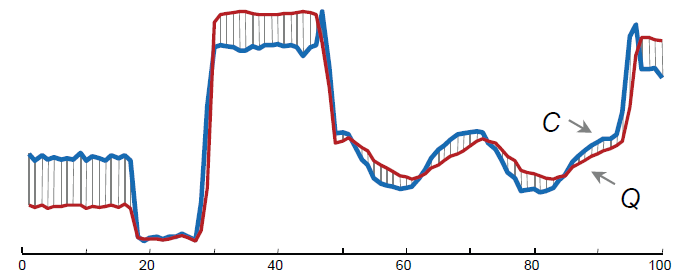
\includegraphics[scale=0.7]{euclidean.png}\\
\vspace*{10pt}
\begin{tabular}{l}
\footnotesize{\textbf{Figura 2.} Visualizaci\'on de la distancia Euclidiana entre dos series temporales C y Q.}\\ 
\end{tabular}{}
\textbf{Fuente:} \cite{euclidean}.
\end{center}
\subsubsection{\textbf{Distancia \enquote{Swale}}}
En \cite{swale}, los autores proponen un modelo de similitud llamado \textbf{\textit{\enquote{Swale}}} (\enquote{\textit{Sequence Weighted ALignmEnt}}, por sus siglas en Ingl\'es); este modelo utiliza un sistema de puntuaci\'on para recompensar las similitudes y penalizar las disimilitudes durante la comparaci\'on de series temporales. El uso del marco de trabajo \textit{Swale}, requiere necesariamente del ajuste de tres par\'ametros: 1- un umbral de similitud \textbf{$\epsilon$}, 2- un valor o peso $r$ utilizado para recompensar las similitudes y 3- un valor o peso $p$ para penalizar los vacios o disimilitudes \cite{swale}.\par
M\'as formalmente, la funci\'on de similitud de \textit{Swale} puede definirse como:\\
Sean R y S dos series de tiempo de longitud m y n, respectivamente. Sea el costo de la diferencia o disimilitud $gap_c$ y el costo de la similitud $reward_m$. Entonces dadas dos series temporales $R$ y $S$,\\
$Swale(R, S) =$
\[
\begin{dcases}
    {n * gap_c},&   \text{if m = 0}\\
    {m * gap_c},&   \text{if n = 0}\\
    {reward_m + },& \text{if }{\forall d, |r_d,1 - S_d,1| \leq \epsilon}\\   
    {Swale(Rest(R), Rest(S)),}\\
    {max\{gap_c + Swale(Rest(R),S)}, & \text{otherwise}\\
    {gap_c + Swale(R, Rest(S))}\} 
\end{dcases}
\]
El modelo Swale, posee una carater\'istica muy particular, ya que permite ajustar los pesos o los valores utilizados para castigar la disimilitud o bien, en sentido contrario, recompensar la similitud, con base en el criterio de un experto con conocimientos muy espec\'ificos de cierto dominio. Esto permite afinar la funci\'on de distancia explicada en la f\'ormula anterior, de manera tal, que pueda establecerse un rendimiento \'optimo con base en la naturaleza de los datos, en lugar de tener una \'unica t\'ecnica para cada dominio de datos \cite{swale}.
\subsubsection{\textbf{Medida de distancia SpADe}}
En \cite{spade}, se define Spatial Assembling Distance
(SpADe por sus siglas en Ingl\'es), como una medida de distancia cap\'az de manejar el desplazamiento y la amplitud en dimensiones de amplitud y tiempo. Adicionalmente, proponen una propuesta eficiente para la detecci\'on continua de patrones, utilizando SpADe, para evaluar la similitud de subsecuencias de series temporales sobre el flujo de datos.\par
Esta medida de distancia basa en la detecci\'on de la mejor combinaci\'on de un patr\'on de similitud local (Local Pattern Match LPM), mediante el c\'alculo de la ruta m\'as corta en la matriz de similitud.\par 
En la siguiente figura, se muestra un ejemplo del c\'omputo de LPM para dos segmentos de series de tiempo Q y D, en condiciones de desplazamiento y amplitud.
\begin{center}
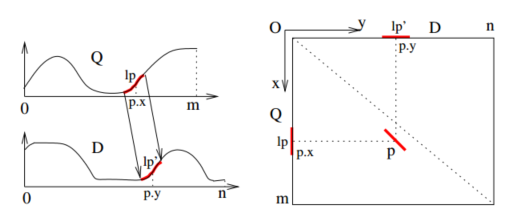
\includegraphics[scale=0.9]{spade.png}\\
\vspace*{10pt}
\footnotesize{\textbf{Figura 3.} Ejemplo del c\'alculo de LPM.}\\ \textbf{Fuente:} \cite{swale}.
\end{center}
SpADe puede definirse matem\'aticamente como:
\begin{equation}
SDl(Dt, Q) = mini<te SD(D[t : i], Q)
\end{equation}
Donde $SDl(Dt, Q)$ mide la distancia de la mejor similitud de la subsecuencia para $(Q)$ iniciando en un punto $t$ con respecto a $D$.\par
En resumen, SpaADe es una medida de distancia robusta basada en \enquote{la forma} de la subsecuencia de la serie temporal. En \cite{spade} se argumentan adem\'as, que no es sensible al desplazamiento o a la amplitud de las dimensiones durante el an\'alisis del flujo de datos de la serie temporal y que por ende, alcanza mejores resultados con respecto a medidas de distancia m\'as comunes tales como distancia Euclidiana o DTW.
\subsubsection{\textbf{Medida de distancia ERP}}
En \cite{erp}, los autores proponen la distancia ERP (\enquote{\textbf{E}dit distance with \textbf{R}eal \textbf{P}enalty} por sus siglas en Ingl\'es). ERP podr\'ia representarse de la siguiente manera, dadas dos series temporales $R$ y $S$,\\
$Swale(R, S) =$
\[
\begin{dcases}
    \sum\limits_{1}^{n}|s_i - g|,&   \text{if m = 0}\\
    \sum\limits_{1}^{m}|r_i - g|,&   \text{if n = 0}\\       
    {min\{ERP(Rest(R), Rest(S)) + dist_{erp}(r_1,s_1)}, & \text{otherwise}\\
    {ERP(Rest(R),S) + dist_{erp}(r_1,gap), RRP(R,Rest(S) + dist_{erp}(S_1,gap)}\} 
\end{dcases}
\]
Donde $g$ es un valor constante, normalmente igual a 0 seg\'un la recomendaci\'on de los autores en \cite{erp}. Los autores, definen ERP como una variante de \textit{L1-norm}, con la excepci\'on de que esta medida de distancia si es capaz de soportar el desplazamiento local en el eje tiempo, en otras palabras, lo autores lo consideran \enquote{el matrimonio perfecto} entre una medidas de distancia \enquote{L1-norm} y una medida de distancia de categor\'ia el\'astica, ya que se asemeja a \enquote{L1-norm} en ser una funci\'on de distancia m\'etrica, pero tambi\'en, se asemeja a distancias el\'asticas como DTW, en su capacidad misma de poder soportar los desplazamientos o transiciones en el eje tiempo \cite{erp}.
\subsubsection{DTW (Dynamic Time Warping)}
En el a\~no 1994, Berndt y Clifford \cite{dtw} proponen \textit{\textbf{\enquote{Dynamic Time Warping}}}. En el an\'alisis de series de tiempo, DTW es un algoritmo para medir el\'asticamente la similitud entre dos secuencias temporales que pueden variar en velocidad y por ende en alineamiento, en relaci\'on con el eje tiempo \cite{concepts}.\par A diferencia de la distancia Euclidiana, el c\'alculo de la similitud no se hace en forma lineal, por el contrario, las secuencias son \enquote{deformadas} de manera no li\-neal, para determinar la medida de similitud independiente con respecto a ciertas variaciones en el eje tiempo \cite{dtw}. Por ejemplo, la tarea de detecci\'on de patrones implica la b\'usqueda de una serie de tiempo $S$, para instancias de una plantilla $T$, donde $S = s_1, s_2, ..., s_i, ..., s_n$ y $T = t_1, t_2, ..., t_i, ..., t_n$.\par
Las secuencias $S$ y $T$, pueden ser acomodadas para conformar un plano de $m$ por $n$ o un cuadrante, en donde cada punto del cuadrante, $(i, j)$, corresponde a un alineamiento entre elementos $s_i$ y $t_i$.\par
Un camino $W$, alinea los elementos que pertenecen a $S$ y a $T$, tal que la distancia entre ellos es minimizada.\\
\begin{equation}
W = w_1, w_2, ..., w_k
\end{equation}
Es decir, $W$ es una secuencia o un camino espec\'ifico de puntos en el cuadrante, en donde cada $w_k$ corresponde a un punto $(i,j)_k$, como se muestra en la figura 3.
\begin{center}
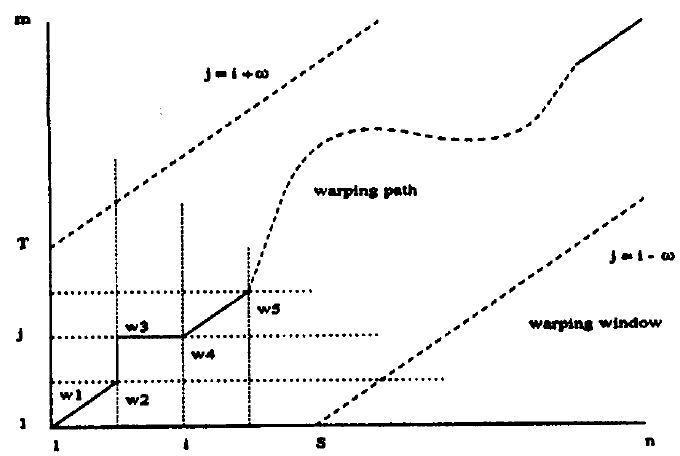
\includegraphics[scale=0.7]{dtw.png}\\
\vspace*{10pt}
\footnotesize{\textbf{Figura 4.} Visualizaci\'on de un camino w en un cuandrante de $m$ por $n$.}\\ \textbf{Fuente:} \cite{dtw}.
\end{center}
Posteriormente, por definici\'on, se debe definir una medida de distancia. En \cite{dtw}, los autores proponen $\delta(i,j) = (s_i - t_j)^2$. Una vez definida la medida de distancia, se puede definir formalmente DTW como la minimizaci\'on sobre los caminos o rutas potenciales \textbf{\textit{no lineales}}, basados en la distancia acumulada para cada ruta, en donde $\delta$ es una medida de distancia entre dos puntos de datos o elementos de las series temporales.
\begin{equation}
DTW (S,T) = min_W[\sum\limits_{k=1}^{p}\delta(w_k)]
\end{equation}
En la Figura 4, se muestra observa un ejemplo claro de la forma que adoptan las deformaciones no lineales calculadas mediante el algoritmo DTW, para adaptar la diferencia de los puntos de datos con respecto al eje tiempo.
\begin{center}
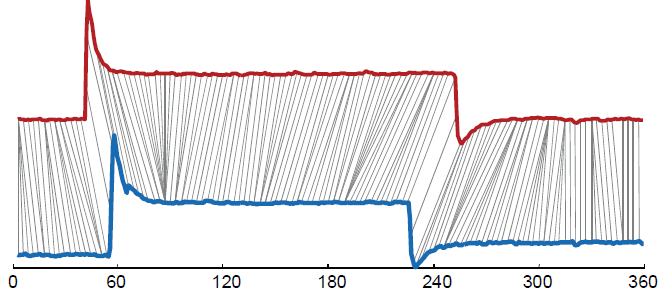
\includegraphics[scale=0.7]{dtw2.png}\\
\vspace*{10pt}
\footnotesize{
\begin{tabular}{l}
\textbf{Figura 5.} Visualizaci\'on de dos segmentos de series temporales
acerca del comportamiento\\ de insectos se alinean con invarianza a la deformaci\'on computada mediante el uso de DTW.
\end{tabular}{}
}
\textbf{Fuente:} \cite{dtw}.
\end{center}
\subsubsection{\textbf{DTW basado en Cubic Spline Interpolation}}
\textbf{D}ynamic \textbf{T}ime \textbf{W}arping basado en Cubic \textbf{S}pline \textbf{I}nterpolation (SIDTW), tambi\'en conocido como \enquote{Cubic Dynamic Time Warping} (CDTW),  fue propuesto recientemente como una novedosa y mejorada extensi\'on de DTW \cite{DTWcubicsplineinterpolation}.\\\\
\textbf{Acerca de la funci\'on SIDTW:}\\
Segun los autores en \cite{DTWcubicsplineinterpolation}, inicialmente, se debe calcular la derivada de cada punto de la series de temporal mediante \enquote{Cubic Spline Interpolation}, a este proceso se le conoce como \enquote{\textbf{interpolaci\'on}}. Lo anterior es necesario para reemplazar las derivadas que fueron estimadas por Derivative Dymanic Time Warping (DDTW). Despu\'es de la interpolaci\'on, se utilizan las secuencias basadas en derivadas para representar las series de tiempo originales, para lograr una mejor descripci\'on la tendencia original de las series temporales, haci\'endolas m\'as f\'acil de deformar (\enquote{warping}) \cite{DTWcubicsplineinterpolation}.\par
En \cite{DTWcubicsplineinterpolation} se argumenta que mediante el uso de esta medida de distancia, se pueden producir menores singularidades (menos \enquote{warping}) y obtener en cambio, la mejor ruta de deformaci\'on posible, con el menor largo. Adem\'as, se considera una versi\'on de medida de distancia alternativa de DTW cuando los conjuntos de datos de las series temporales no son adecuados para ser medidos a trav\'es de DTW \cite{DTWcubicsplineinterpolation}.\par
La principal motivaci\'on de SIDTW como propuesta es en esencia obtener derivadas mucho m\'as precisas para reflejar mejor la tendencia de las series de tiempo que estan siendo comparadas y as\'i, mejorar tambi\'en la efectividad de la medida de similitud para las distancias acumuladas de tres elementos adyacentes \cite{DTWcubicsplineinterpolation}.\par
Por ejemplo,
\[
	{r(i,j) = d(i,j) + min}
\begin{dcases}
    {r(i,j - 1)}	\\
    {r(i - 1,j - 1)}\\
    {r(i - 1,j)}    \\
\end{dcases}
\]
Sin embargo, en DDTW, los pasos son los mismos que en DTW, adem\'as de la diferencia de los cuadrados entre $q_i$ y $c_j$.\par
La estimaci\'on de la derivada $d'(i,j)$ en DDTW es utizada para reemplazar la distancia $d(i,j)$ en DTW. De esta forma, tenemos la siguiente derivada:
\begin{equation}
d'(i,j) = (d_i(q) - d_j(c))^2
\end{equation}
donde, 
\begin{equation}
d_l(x) = \frac{((x_l - x_{l-1}) + (x_{l-1} - x_{l-1})/2)}{2}
\end{equation}
Como se muestra en la siguiente imagen, una de las principales ventajas de CDTW es el hecho de que se pueden evitar la creaci\'on de deformaciones innecesarias.
\begin{center}
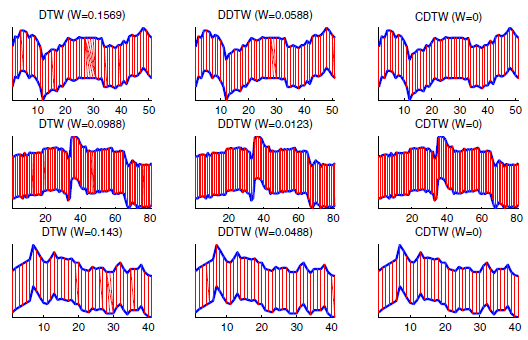
\includegraphics[scale=0.8]{cdtw.png}\\
\vspace*{10pt}
\footnotesize{\textbf{Figura 6.} Visualizaci\'on de deformaciones innecesarias en DTW.} \textbf{Fuente:} \cite{DTWcubicsplineinterpolation}.
\end{center}
En la imagen anterior, $W$ corresponde a la cantidad de deformaciones producidas, en donde para DTW y DDTW, se observan valores mayores zero, mientras que en CDTW no produce deformaciones.\par
Los experimentos sobre conjuntos de datos de series temporales desarrollados en \cite{DTWcubicsplineinterpolation}, reflejan que SIDTW puede reducir significativamente el n\'umero de singularidades y alinear m\'as adecuadamente los puntos entre las dos series de tiempo (facilitando notablemente el c\'omputo de la similitud). En resumen, mientras m\'as precisa sea la pendiente, m\'as efectivo ser\'a tambi\'en el c\'omputo de la deformaci\'on sobre las series de tiempo. Finalmente, cuando existen muchos puntos adyacentes con valores iguales en la serie de tiempo, los autores proponen el uso de \textbf{CDTW}, como una alternativa viable y superior (por ejemplo en comparaci\'on con DTW y DDTW) para evitar la producci\'on de deformaciones innecesarias 	\cite{DTWcubicsplineinterpolation}.
\subsubsection{El Ruido y la Interpolaci\'on en Series Temporales}
La recolecci\'on de los datos de una serie de tiempo se encuentra siempre degradada por ruido en cierto grado \cite{noise}. Incluso una estimaci\'on aproximada del nivel de ruido contenido en la serie temporal es crucial, previo al an\'alisis de los datos.\par
En la pr\'actica, las series de tiempo no estacionarias son muy comunes en campos diversos como la geof\'isica, las finanzas y las ciencias biol\'ogicas \cite{concepts}.\par
En el siguiente gr\'afico se pueden observar, por ejemplo, segmentos \textit{no estacionarios} de se\~nales de un electroencefalograma a partir de la medici\'on clinica intracraneal de un individuo \cite{noise}.
\begin{center}
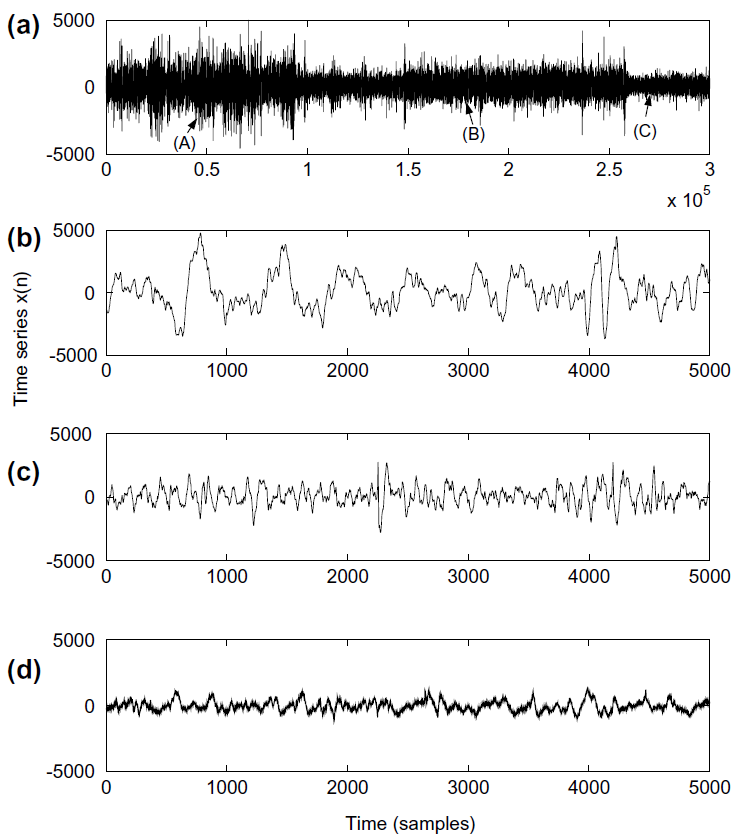
\includegraphics[scale=0.7]{brainsignal.png}\\
\vspace*{10pt}
\footnotesize{\textbf{Figura 7.} Medici\'on Cl\'inica Intracraneal. Visualizac\'ion de ruido.}\\ \textbf{Fuente:} \cite{noise}.
\end{center}
En la figura 7, se puede apreciar la presencia de ruido en la serie temporal \textbf{(a)}. Es posible tambi\'en, observar los segmentos subyacentes \textbf{(b)}, \textbf{(c)} y \textbf{(d)}, superposicionados como parte de \textbf{a} y luego evaluados como segmentos individuales, con a\'un presencia de \enquote{\textit{\textbf{ruido blanco}}}.\par
El ruido blanco es una se\~nal aleatoria (conocida tambi\'en como proceso estoc\'astico) que se caracteriza por el hecho de que sus valores en el eje tiempo, no guardan correlaci\'on estad\'istica. En resumen, el ruido blanco es no correlativo, es decir, en el eje del tiempo la se\~nal toma valores sin ninguna relaci\'on unos con otros \cite{concepts}.\par
Matem\'aticamente, podr\'ia definirse entonces como una sucesi\'on de variables aleatorias (procesos estoc\'astico) con una esperanza (media) cero y una varianza constante e independientes de cualquier valor de t (covarianza nula) \cite{noise}.\par
Los valores faltantes, al igual que el ruido, representan igualmente un problema serio que debe abordarse previo al an\'alisis de series temporales.\par
La interpolaci\'on por su parte, es un concepto que puede ser aplicado a los datos de series temporales para determinar valores faltantes. En primera instancia, se debe comprender el modelo de datos apropiado con el que se esta trabajando (autorregresivo, autorregresivo de media m\'ovil, autorregresivo integrado de media m\'ovil o lineal). Una vez definido el modelo y de acuerdo con la posici\'on de la observaci\'on faltante, se deben calcular las ponderaciones apropiadas para hacer un pron\'ostico en ambas direcciones, hacia adelante o hacia atr\'as. Finalmente, utilizando una combinaci\'on lineal del pron\'ostico anterior, se podr\'an predecir entonces los valores faltantes bajo las condiciones dadas \cite{concepts}.